\documentclass[a4paper,11pt,twocolumn]{article}

% Essential Packages
\usepackage[T1]{fontenc}
\usepackage[utf8]{inputenc}
\usepackage{lmodern}
\usepackage[top=1cm, bottom=2cm, right=1cm, left=1cm, columnsep=1cm]{geometry}

% Math & Logic
\usepackage{amsmath, amsfonts, amssymb, amsthm}
\usepackage{ebproof}
\usepackage{cancel}
\usepackage{mathrsfs}

% Formatting & Layout
\usepackage[skip=10pt]{parskip} 
\usepackage{enumitem} 
\usepackage{array}
\usepackage{xcolor}
\usepackage{tcolorbox}
\usepackage[colorlinks=true, urlcolor=blue]{hyperref}

% Date & Time
\usepackage[nodayofweek, 12hr]{datetime} % 

% Graphics
\usepackage{tikz}
\usetikzlibrary{automata, positioning} 

\usepackage{pdflscape}

% Custom Commands
\newcommand{\limplies}{\rightarrow}
\newcommand{\lequivalent}{\iff}
\newcommand{\ltautology}{\mathbb{T}}
\newcommand{\lcontradiction}{\mathbb{F}}
\newcommand{\ZZ}{\mathbb{Z}}
\newcommand{\RR}{\mathbb{R}}
\newcommand{\NN}{\mathbb{N}}

\newcommand*\circled[1]{\tikz[baseline=(char.base)]{\node[shape=circle,draw,inner sep=2pt] (char) {#1};}}


\begin{document}
	\begin{center}
		{
			\LARGE \textsc{Cosc}264: My Test Summery Sheet
		}
		
		{
			\small Thomas Booker \quad 56118260
		
			\small Compiled on \today{} at \currenttime{}
			
			Test on the 14\textsuperscript{th} September (Week 8) at 6:30pm in JE233
		} 
		\rule{\linewidth}{0.4pt}
	\end{center}
	
	\small
	
\section*{Manchester}
	
\begin{center}
\begin{tikzpicture}[scale=2]
	%\draw[right] (1.1,0) node {Time};
	%\draw[above] (0,1.1) node {Level};
	\foreach \i in {0,...,1} {
		\draw [thin, dashed] (\i,-0.1) -- (\i,1.1);
		%\draw [below] (\i,-0.1) node {$\i$};
	}
	\foreach \i in {0,...,1} {
		\draw [thin, dashed] (-0.1,\i) -- (1.1,\i);
	}
	\draw [left] (-0.1,0) node {-V};
	\draw [left] (-0.1,1) node {+V};
	
	\draw[-, very thick] (0,0) -- (0.5,0) -- (0.5,1)-- (1,1);
	\draw[above] (0.5,1.1) node {\Large \textbf{0}};
	
	% ---
	
	\foreach \i in {2,...,3} {
		\draw [thin, dashed] (\i,-0.1) -- (\i,1.1);
		%\draw [below] (\i,-0.1) node {$\i$};
	}
	\foreach \i in {0,...,1} {
		\draw [thin, dashed] (2-0.1,\i) -- (3.1,\i);
	}
	
	\draw[-, very thick] (2,1) -- (2.5,1) -- (2.5,0)-- (3,0);
	\draw[above] (2.5,1.1) node {\Large \textbf{1}};
	
\end{tikzpicture}
\end{center}

\section*{Differential Manchester}

In Differential Manchester, the signal always flips at t=0.5.

If a 1 is encountered in the digital data, no signal flip is generated at t=0.

If a 0 is encountered in the digital data, a signal flip is generated at t=0.

\begin{center}
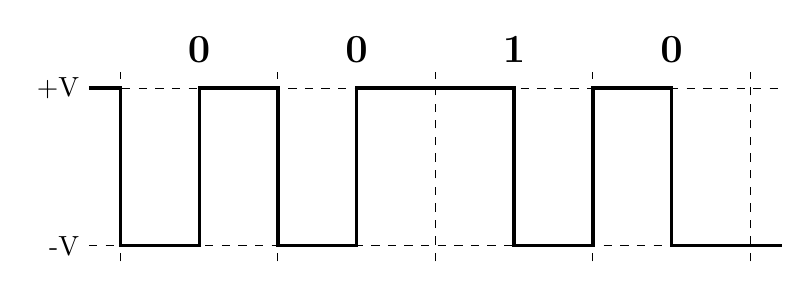
\begin{tikzpicture}[scale=2]
	%\draw[right] (1.1,0) node {Time};
	%\draw[above] (0,1.1) node {Level};
	\foreach \i in {0,...,4} {
		\draw [thin, dashed] (\i,-0.1) -- (\i,1.1);
		%\draw [below] (\i,-0.1) node {$\i$};
	}
	\foreach \i in {0,...,1} {
		\draw [thin, dashed] (-0.2,\i) -- (4.2,\i);
	}
	\draw [left] (-0.2,0) node {-V};
	\draw [left] (-0.2,1) node {+V};
	
	\draw[-, very thick] (-0.2,1) -- (0,1) -- (0,0) -- (0.5,0) -- (0.5,1) -- (1,1) -- (1, 0) -- (1.5, 0) -- (1.5,1) -- (2,1) -- (2.5,1) -- (2.5,0) -- (3,0) -- (3,1) -- (3.5,1) -- (3.5,0) -- (4.2,0);
	\draw[above] (0.5,1.1) node {\Large \textbf{0}};
	\draw[above] (1.5,1.1) node {\Large \textbf{0}};
	\draw[above] (2.5,1.1) node {\Large \textbf{1}};
	\draw[above] (3.5,1.1) node {\Large \textbf{0}};
	
\end{tikzpicture}
\end{center}

\section*{Analog Carrier + Digital Data}
\[ s(t) = A(t)\cdot\cos\left(\left(f_c+f(t)\right)\cdot t+\phi(t)\right) \]
\begin{center}
	\begin{tabular}{cl}
		$s$ & Signal \\
		$A$ & Amplitude \\
		$f_c$ & Center frequency \\
		$f$ & Frequency offset \\
		$\phi$ & Phase (wave offset) \\
	\end{tabular}
\end{center}
\begin{description}
	\item[PSK] Phase-shift keying
	\[ s(t) = A\cdot\cos\left(f_c\cdot t+\phi(t)\right) \]
	\item[FSK] Frequency-shift keying
	\[ s(t) = A\cdot\cos\left(\left(f_c+f(t)\right)\cdot t\right) \]
	\item[ASK] Amplitude-shift keying
	\[ s(t) = A(t)\cdot\cos\left(f_c\cdot t\right) \]
\end{description}
\subsection*{Example Diagrams}
\begin{center}
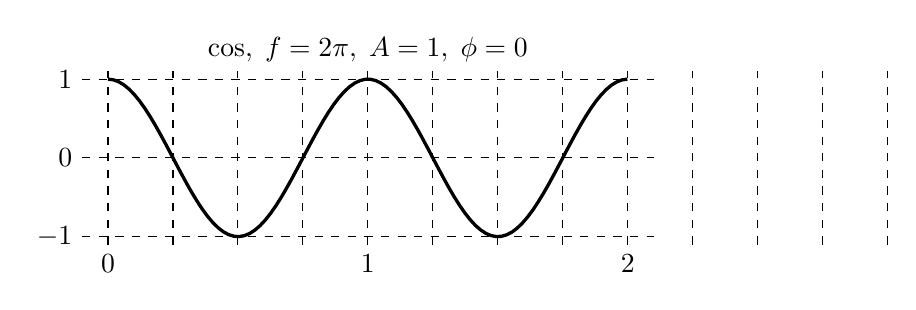
\begin{tikzpicture}[yscale=1,xscale=3.3]
	\foreach \i in {0,0.25,...,3} {
		\draw [thin, dashed] (\i,-1.1) -- (\i,1.1);
	}
	\foreach \i in {0,...,2} {
		\draw [below] (\i,-1.1) node {$\i$};
	}
	\foreach \i in {-1,...,1} {
		\draw [thin, dashed] (-0.1,\i) -- (2.1,\i);
		\draw [left] (-0.1,\i) node {$\i$};
	}
	
	\draw[above] (1,1.1) node {$\cos,\; f=2\pi,\; A=1,\;\phi=0$};
	\draw[-,very thick,domain=0:2,samples=100] plot (\x, {cos(\x * 360)});
\end{tikzpicture}

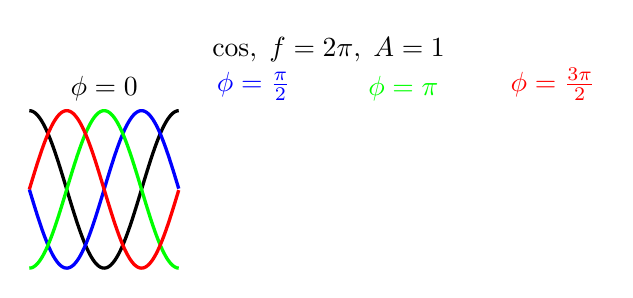
\begin{tikzpicture}[yscale=1,xscale=1.9]

	\draw[above] (2,1.5) node {$\cos,\; f=2\pi,\; A=1$};
	\draw[above] (0.5,1) node {$\phi=0$};
	\draw[above, blue] (1.5,1) node {$\phi=\frac{\pi}2$};
	\draw[above, green] (2.5,1) node {$\phi=\pi$};
	\draw[above, red] (3.5,1) node {$\phi=\frac{3\pi}2$};
	\draw[-,very thick,domain=0:1,samples=100] plot (\x, {cos(\x * 360)});
	\draw[-,very thick,domain=0:1,samples=100, blue] plot (\x, {cos(\x * 360 + 90)});
	\draw[-,very thick,domain=0:1,samples=100, green] plot (\x, {cos(\x * 360 + 180)});
	\draw[-,very thick,domain=0:1,samples=100, red] plot (\x, {cos(\x * 360 + 270)});
\end{tikzpicture}

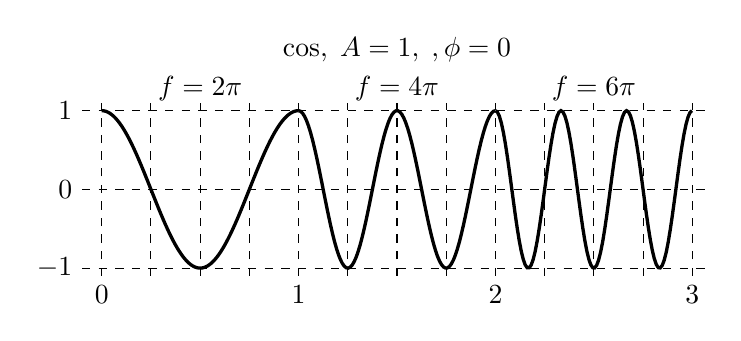
\begin{tikzpicture}[yscale=1,xscale=2.5]
	\foreach \i in {0,0.25,...,3} {
		\draw [thin, dashed] (\i,-1.1) -- (\i,1.1);
	}
	\foreach \i in {0,...,3} {
		\draw [below] (\i,-1.1) node {$\i$};
	}
	\foreach \i in {-1,...,1} {
		\draw [thin, dashed] (-0.1,\i) -- (3.1,\i);
		\draw [left] (-0.1,\i) node {$\i$};
	}
	
	\draw[above] (1.5,1.5) node {$\cos,\; A=1,\;,\phi=0$};
	\draw[above] (0.5,1) node {$f=2\pi$};
	\draw[above] (1.5,1) node {$f=4\pi$};
	\draw[above] (2.5,1) node {$f=6\pi$};
	\draw[-,very thick,domain=0:1,samples=100] plot (\x, {cos(\x * 360)});
	\draw[-,very thick,domain=1:2,samples=100] plot (\x, {cos(\x * 2 * 360)});
	\draw[-,very thick,domain=2:3,samples=100] plot (\x, {cos(\x * 3 * 360)});
\end{tikzpicture}
\end{center}
\section*{Medium Access Control (MAC)}
Broadcast/Shared medium, transmission are heard by all stations. If two transmissions overlap, both are garbled (Not true in some system we don't talk about).

Orthogonal Schemes: Split a chancel into smaller sub-chancel that can be transitioned on without collation between the sub-chancels.

The \textbf{medium access delay} is the time a station must wait to start transmitting (access the medium).

\subsection*{Frequency Division Multiple Access (FDMA)}

The given channel bandwidth is subdivided into $N$ sub-channels. Guard bands: reduction of adjacent-channel interference, robustness against imperfect frequency synchronisation. Access Delay is 0.


\subsection*{Time Division Multiple Access (TDMA)}

Time is subdivided into superframes of duration $T_{SF}$.
Each superframe is subdivided into $N$ time-slots.
There are short guard times between time slots.

Neglecting guard times, each sub-chancel gets the full channel bandwidth for a fraction $\frac1N$ of the time. So, the bit rate for a sub-chancel is $\frac BN$. The average medium access delay for one sub-chancel is $E\left[\text{Access Delay}\right]=\frac{T_{SF}}{2}$.

\subsection*{Random Access Protocols}

Random access protocols: \\
Do not attempt to reserve channel resources for long times. \\
Do not require a central station or (much) shared state. \\
Do not access the medium at predictable times. \\
Often have low complexity (e.g. little coordination, if any). \\
Typically involve some random element.

Random access protocols accept risk of collisions to save coordination
overhead and have overall improved efficiency! How well this trade-off
works depends for example on the offered traffic load.

\subsection*{Pure ALOHA}

Uses checksum to drop garbled packets. All packets are transmitted immediately with no coordination. Upon transmission a acknowledgement timer is started. The receiver sends an immediate ack upon successful reception (without a collision or transmission error); If not successful, the receiver remains quiet. If the transmitter receives an ack before the ack timeout, the frame is forgotten and the ack timer is cancelled. If the ack timer expires, transmitter enters a backoff mode: A random amount of time is waited and then the packet is re-transmitted. If the number of failed re-transmission trials exceeds threshold, the frame is dropped. New packets ready for transmission will wait in a queue if the station is backlogged.

The vulnerability period is 2 times the frame length. When more stations are active the collision probability increases. ALOHA cannot distinguish between collisions and channel errors destroying a frame.

\subsection*{Carrier Sense Multiple Access (CSMA)}

All stations can determine the state of the medium (almost) instantaneously. Called carrier-sensing (CS) or clear-channel assessment.

Listen-before-talk (LBT): Before station transmits a frame, it performs CS operation. If channel is busy, station defers transmission according to one of
several possible strategies.

CSMA protocols do not eliminate collisions completely, but reduce
their rate or their impact. 

CSMA approach is especially useful when medium propagation time is small compared to packet length, since other stations notice transmission quickly after it started. Typically satisfied in LANs, propagation delay is small
Collisions can only occur when two stations start transmitting at almost same time (time difference smaller than propagation delay).

When propagation time is large compared to packet length, the
sender might have already stopped transmission when receiver
senses an idle carrier for the first time. Example: multi-access satellite configurations. Here LBT is almost useless, ALOHA is reasonable.

\end{document}
